\documentclass[a4paper]{article}
\usepackage[english]{babel}
\usepackage[utf8]{inputenc}
\usepackage{amsmath}
\usepackage{multirow}
\usepackage{graphicx}
% \graphicspath{ {images/} }
%\usepackage[colorinlistoftodos]{todonotes}

\title{CS771A Project Report : Assignment1  }

\author{ \hspace{0.1cm}Siddhant Manocha \\
        Roll 12714 \\
        }

\date {\today} 

\begin{document}

\maketitle


\section{Determining the Model for Classification}
In the given assignment , we were asked to use Pima Indian Diabetes for prediction of diabetes among patients. The dataset has in total 768 data points and we use five fold cross validation to report our prediction results.
\\
In order to build the model, we consider the following criterions \\
\begin{itemize}
\item Threshold the tree based on decrease in impurity value at the node
\item Threshold on the number of nodes for a particular split or number of data vectors required at the node for the split
\item Growing the complete tree and then pruning the tree
\item Considering different impurity functions as gini and information(entropy)
\end{itemize} 

We did 5 fold cross validation to determine the optimum value for various parameters.
\begin{itemize}
\item To set a threshold on the number of decrease in impurity, we iterated over values from 0 to 0.2 over a step size of 0.001 and found the threshold that maximizes the average accuracy over cross validation.
\item To set threshold on number of nodes in split, we iterated over values from 0 to 150 to find its optimum value
\item For pruning we iterated over values of the complexity parameter, which determines the extent upto which the tree will be pruned and determined its optimum value
\end{itemize} 


\section{Handling the Missing Data}
In the given dataset, a lot of values were missing. In this case, missing values were not externally specified but the values were absurd for a given field.
We considered the zero values in column 2,3,4,5,6 , namely amount of plasma glucose, blood pressure, triceps skin thickness, serum insulin, etc as the absurd values and replaced them by NA and handled them accordingly.

Steps taken for handling the missing values.
 \\
Test Set:
\begin{itemize}
\item Avoid missing attributes and perform impurity calculation by not considering the attributes if the value was missing
\item Replace the missing values in positive examples by the mean of non missing samples having positive label and vice versa
\item Replace the missing values in positive examples by the median of non missing samples having positive and vice versa
\item Replace missing values by class based mean for the whole dataset
\end{itemize} 

Training Set:
\begin{itemize}
\item Build surrogate splits at each node and make predictions on the basis the surrogate splits in case of missing attributes 
\item Replace the test data by the overall mean of the training data
\item Replace the test data by the overall median of the training data
\item Replace the missing values by class based means for the whole dataset
\end{itemize} 


\section{Results}
\subsection{Case1}
Description: Do not replace the missing data in training. Use surrogate splits for testing.
\begin{itemize} 
\item Threshold on number of nodes.Impurity function: information\\
Accuracy: 76.95357 \%  \\
Optimum Split: 23

\item Threshold on decrease in impurity.Impurity function: information\\
Accuracy: 76.16\%  \\
Optimum threshold: 0.031 \%

\item Threshold on complexity parameter for pruning.Impurity function: information\\
Accuracy: 73.57 \%  \\
Optimum threshold:0.02

\item Threshold on number of nodes.Impurity function: gini\\
Accuracy: 76.17 \%  \\
Optimum Split: 94

\item Threshold on decrease in impurity.Impurity function: gini\\
Accuracy: 75.12\%  \\
Optimum threshold: 0.011 \%

\item Threshold on complexity parameter for pruning.Impurity function: gini\\
Accuracy: 74.877 \%  \\
Optimum threshold:0.04

\subsection{Case2}
Description:Replace the missing values by the class based(positive and negative) mean for the whole dataset .

\item Threshold on number of nodes.Impurity function: gini\\
Accuracy: 87.50  \%  \\
Optimum Split: 36 

\item Threshold on decrease in impurity.Impurity function: gini\\
Accuracy: 88.28 \%  \\
Optimum threshold: 0.058

\item Threshold on complexity parameter for pruning.Impurity function: gini\\
Accuracy: 86.33 \%  \\
Optimum threshold: 0.02


\subsection{Case3}
Description:Replace the missing values by the class based(positive and negative) medians for the whole dataset .


\item Threshold on decrease in impurity.Impurity function: gini\\
Accuracy: 87.88\%  \\
Optimum Split: 24 \%

\item Threshold on complexity parameter for pruning.Impurity function: gini\\
Accuracy: 86.84 \%  \\
Optimum Split:0.016

\item Threshold on number of nodes.Impurity function: gini\\
Accuracy: 85.54 \%  \\
Optimum Split: 0.02


\subsection{Case4}
Description:Replace the missing values in training by class based mean and testing set by mean of the training set


\item Threshold on decrease in impurity.Impurity function: information\\
Accuracy: 67.20\%  \\
Optimum Split: 0.016 \%

\item Threshold on complexity parameter for pruning.Impurity function: information\\
Accuracy: 68.61\%  \\
Optimum Threshold:0.077

\item Threshold on number of nodes.Impurity function: information\\
Accuracy: 65.10  \%  \\
Optimum Threshold: 0.58




\end{itemize} 

\section{Submission}
For given assignment , I have submitted two files: hw\_test.R and hw\_test2.R  \\
In hw\_test.R :I have parameters: n\_fold which specifies the fold for validation  \\
thresholdtype : 1) for split size 2) decrease in impurity 3) pruning \\
impurity function : gini or information ,replace by : none , mean , median which specifies whether to replace data by mean , median or no change  \\
Similarly for hwtest\_2.R, except we can explicitly mention how to handle missing data for the test and the training

\section{Comments}
The best accuracy is achieved in case when the missing data is replaced by the mean of the overall data for the testing data as well as the training data. But such an approach may overfit our data and thus reports unexpectedly high accuracies.In case of using suurogate splits, results are reasonable and gives better results for missing data against using means to replace the data for training and testing seperately.


\section{Tree Diagrams}

\begin{figure}[ht!]
\centering
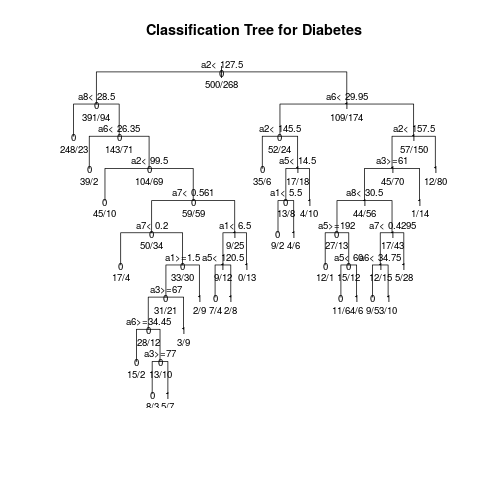
\includegraphics[width=90mm]{images/tree.png}
\caption{Full grown Tree \label{overflow}}
\end{figure}

\begin{figure}[ht!]
\centering
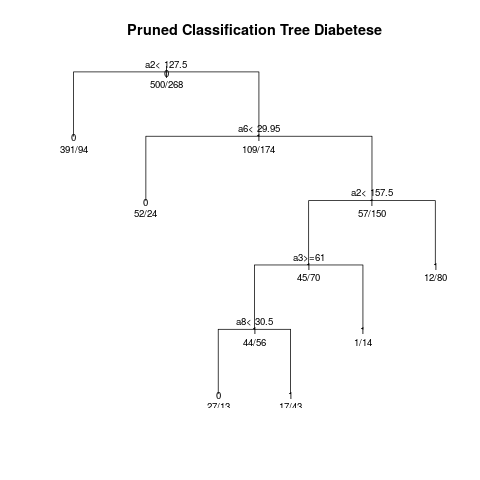
\includegraphics[width=90mm]{images/ptree.png}
\caption{Pruned Tree at optimum complexity parameter \label{overflow}}
\end{figure}



\end{document}
